% Genera: sistema_control_componentes.svg  (en ../img_gen/)
% Estilo: diagrama de bloques B/N estilo LaTeX/Ogata.
% Compilar:
%   pdflatex sistema_control_componentes.tex
%   pdf2svg sistema_control_componentes.pdf ../img_gen/sistema_control_componentes.svg
\documentclass[border=6pt]{standalone}
\usepackage{tikz}
\usepackage{amsmath}
\usetikzlibrary{arrows.meta, positioning, calc}
\begin{document}
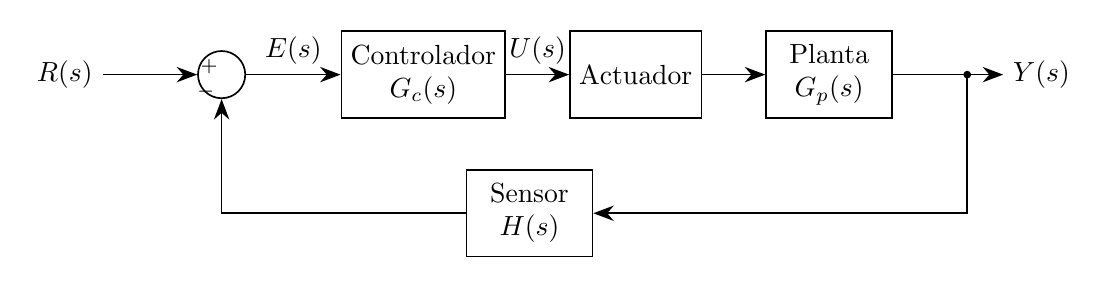
\begin{tikzpicture}[
    >={Stealth[length=2.6mm]},
    line width=0.6pt,
    block/.style={draw, rectangle, minimum height=11mm, minimum width=16mm, align=center},
    sum/.style={draw, circle, minimum size=6mm, inner sep=0pt},
    node distance=10mm
  ]
  % --- rama directa ---
  \node (in)    {$R(s)$};
  \node[sum, right=12mm of in] (sum) {};
  \node[block, right=12mm of sum] (ctrl) {Controlador\\ $G_c(s)$};
  \node[block, right=8mm of ctrl] (act)  {Actuador};
  \node[block, right=8mm of act]  (plant){Planta\\ $G_p(s)$};
  \node[right=14mm of plant] (out) {$Y(s)$};
  \coordinate (pick) at ($(plant.east)!0.5!(out)$);

  % --- sensor en realimentacion ---
  \node[block, below=12mm of $(ctrl)!0.5!(act)$] (sensor) {Sensor\\ $H(s)$};

  % --- conexiones ---
  \draw[->] (in) -- (sum);
  \draw[->] (sum) -- node[above]{$E(s)$} (ctrl);
  \draw[->] (ctrl) -- node[above]{$U(s)$} (act);
  \draw[->] (act) -- (plant);
  \draw[->] (plant) -- (out);
  \fill (pick) circle (1.4pt);
  \draw[->] (pick) |- (sensor.east);
  \draw[->] (sensor.west) -| (sum);

  % --- signos del sumador ---
  \node at ($(sum.north west)+(0.6mm,-1.2mm)$) {\scriptsize $+$};
  \node at ($(sum.south)+(-2.0mm,1.0mm)$) {\scriptsize $-$};
\end{tikzpicture}
\end{document}
